\documentclass[10pt,a4paper]{article}
\usepackage[margin=0.5in]{geometry}
\usepackage[utf8]{inputenc}
\usepackage[english]{babel}
\usepackage{amsmath}
\usepackage{amsfonts}
\usepackage{amssymb}
\usepackage{cancel}
\usepackage{xcolor}
\usepackage{graphicx}

%\renewcommand\CancelColor{<color command>}
\newcommand\cc[2][black]{\renewcommand\CancelColor{\color{#1}}\cancel{#2}}
\newcommand{\ud}[1]{\underline{#1}}
\DeclareMathOperator{\tm}{\times}
\DeclareMathOperator{\A}{\ud{A}}
\DeclareMathOperator{\B}{\ud{B}}
\DeclareMathOperator{\C}{\ud{C}}
\DeclareMathOperator{\G}{\ud{G}}
\DeclareMathOperator{\av}{\ud{a}}
\DeclareMathOperator{\bv}{\ud{b}}
\DeclareMathOperator{\cv}{\ud{c}}


\title{Solid angle subtended by a tetrahedron computation}
\begin{document}

\maketitle


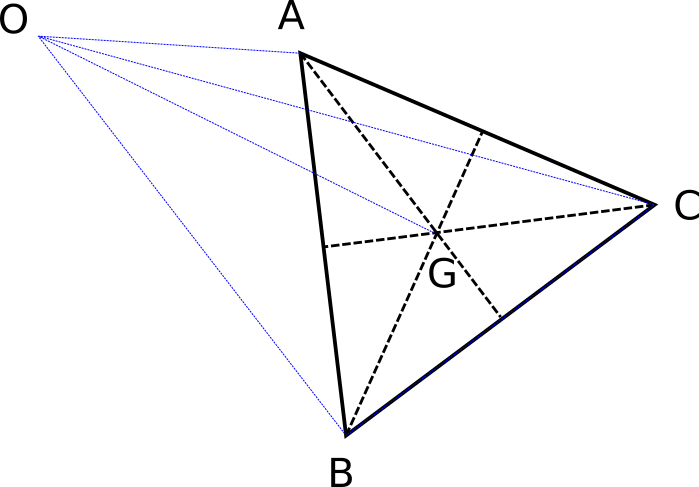
\includegraphics[scale=0.4]{tetra.png} 


\section{Notations}

\subsection{vectors}

\begin{itemize}
	\item $\A=\vec{OA}$
	\item $\B=\vec{OB}$
	\item $\C=\vec{OC}$
	\item $\G=\vec{OG}$
	\item $\av=\vec{GA}$
	\item $\bv=\vec{GB}$
    \item $\cv=\vec{GC}$
\end{itemize}

\subsection{scalars}

\begin{itemize}
	\item $A = \|\A\|$
	\item $B = \|\B\|$
	\item $C = \|\C\|$
	\item $a = \|\av\|$
	\item $b = \|\bv\|$
	\item $c = \|\cv\|$
\end{itemize}

\section{Computation}

The solid angle $\Omega$ subtended by the triangular surface $ABC$ is:

$$
{\displaystyle \tan \left({\frac {1}{2}}\Omega \right)
  = {\frac {\left|{\A}\ {\B}\ {\C}\right|}
    {ABC + \left({\A}\cdot {\B}\right)C
      + \left({\A}\cdot {\C}\right)B
      + \left({\B}\cdot {\C}\right)A}}}
$$

where $ \left|{\A}\ {\B}\ {\C}\right| = {\A}\cdot ({\B}\tm {\C}) $


\subsection{Numerator}


Given that $\A = \G + \av$ (and resp.
with $\B$ and $\C$), we get


\begin{align*}
\left|{\A}\ {\B}\ {\C}\right|
    & =& {\A} \cdot ({\B}\tm {\C}) \\
    & =&  {(\G + \av)} \cdot ({(\G + \bv)} \tm {(\G + \cv)}) \\
    & =&  {(\G + \av)} \cdot (\cancel{\G \tm \G}
	                      + \G \tm \cv
	                      + \bv \tm \G
	                      + \bv \tm \cv) \\
    & =& \cancel{\G \cdot (\G \tm \cv)}
	                      + \cancel{\G \cdot (\bv \tm \G)}
                          + \G \cdot (\bv \tm \cv)
      + \av \cdot (\G \tm \cv)
	  + \av \cdot (\bv \tm \G)
	  + \cancel{\av \cdot (\bv \tm \cv)} \\
    & =& \G \cdot (\bv \tm \cv)
	+ \G \cdot (\cv \tm \av)
	+ \G \cdot (\av \tm \bv) \\
    & = &\G \cdot \left(\bv \tm \cv
	+ \cv \tm \av
	+ \av \tm \bv \right)
\end{align*}

since $G$ is the centroid of $ABC$, 

\begin{equation}
\av + \bv + \cv= 0
\label{eq1}
\end{equation}. We obtain

\begin{align}
\left|{\A}\ {\B}\ {\C}\right|
& = \G \cdot \left(\bv \tm \cv + \cv \tm \av + \av \tm \bv \right) \nonumber \\
& = \G \cdot \left(\bv \tm \cv + \cv \tm (-\bv-\cv)	+ (-\bv-\cv) \tm \bv \right) \nonumber \\
& = \G \cdot \left(\bv \times \cv + \cv \times (-\bv) + \cancel{\cv \times (-\cv)}
	+ \cancel{(-\bv) \times \bv} + (- \cv) \times \bv \right) \nonumber \\
& = \G \cdot \left(3 \bv \times \cv \right) \nonumber \\
& = 3 \G \cdot \left( \bv \times \cv \right)
\end{align}


\subsection{norms}

We can write:
$$
\begin{array}{ll}
    A^2
    & = \A \cdot \A\\
    & = (\G+\av) \cdot (\G + \av)\\
    & = G^2 + 2\G \cdot \av + a^2\\
\end{array}
$$

Hence:
$$
\begin{array}{ll}
    (ABC)^2
    & = (G^2 + 2\G \cdot \av + a^2)
    (G^2 + 2\G \cdot \bv + b^2)
    (G^2 + 2\G \cdot \cv + c^2)\\
    & = (G^2 + 2\G \cdot \av + a^2)
    (G^4 + 2G^2\G \cdot \cv + G^2c^2
     + 2G^2\G \cdot \bv + 4(\G \cdot \bv)(\G \cdot \cv) + 2c^2\G \cdot \bv
     + b^2G^2 + 2b^2\G \cdot \cv + b^2c^2)\\
\end{array}
$$

Given that: $\av = -(\bv+\cv) \Rightarrow a^2=b^2 + 2\bv \cdot \cv + c^2$

We can write:
$$
\begin{array}{lll}
    (ABC)^2
    & = & (G^2 + 2\G \cdot \av + a^2)
    (G^4 + 2G^2\G \cdot \cv + G^2c^2
     + 2G^2\G \cdot \bv + 4(\G \cdot \bv)(\G \cdot \cv) + 2c^2\G \cdot \bv
     + b^2G^2 + 2b^2\G \cdot \cv + b^2c^2)\\
    & = & (G^2 - 2\G \cdot \bv - 2\G \cdot \cv + b^2 + 2\bv \cdot \cv + c^2)\\
    && (G^4 + 2G^2\G \cdot \cv + G^2c^2
     + 2G^2\G \cdot \bv + 4(\G \cdot \bv)(\G \cdot \cv) + 2c^2\G \cdot \bv
     + b^2G^2 + 2b^2\G \cdot \cv + b^2c^2)\\
    & = & G^2
    \left(G^4 + \cc[black]{2G^2\G \cdot \cv} + G^2c^2
     + \cc[red]{2G^2\G \cdot \bv} + \cc[blue]{4(\G \cdot \bv)(\G \cdot \cv)}
     + \cc[green]{2c^2\G \cdot \bv}
     + b^2G^2 + \cc[yellow]{2b^2\G \cdot \cv} + b^2c^2\right)\\
     && - 2\G \cdot \bv
    \left(\cc[red]{G^4} + \cc[blue]{2G^2\G \cdot \cv} + \cc[green]{G^2c^2}
     + 2G^2\G \cdot \bv + 4(\G \cdot \bv)(\G \cdot \cv) + 2c^2\G \cdot \bv
     + \cc[red]{b^2G^2} + \cc[cyan]{2b^2\G \cdot \cv} + \cc[blue]{b^2c^2}\right)\\
     && - 2\G \cdot \cv 
    \left(\cc[black]{G^4} + 2G^2\G \cdot \cv + \cc[magenta]{G^2c^2}
     + 2G^2\G \cdot \bv + 4(\G \cdot \bv)(\G \cdot \cv)
     + \cc[black]{2c^2\G \cdot \bv}
     + \cc[yellow]{b^2G^2} + 2b^2\G \cdot \cv + \cc[green]{b^2c^2}\right)\\
     &&+ 2\bv \cdot \cv
    \left(G^4 + 2G^2\G \cdot \cv + G^2c^2
     + 2G^2\G \cdot \bv + 4(\G \cdot \bv)(\G \cdot \cv) + 2c^2\G \cdot \bv
     + b^2G^2 + 2b^2\G \cdot \cv + b^2c^2\right)\\
     && + b^2
    \left(G^4 + 2G^2\G \cdot \cv + G^2c^2
     + \cc[red]{2G^2\G \cdot \bv} + \cc[cyan]{4(\G \cdot \bv)(\G \cdot \cv)}
     + \cc[blue]{2c^2\G \cdot \bv}
     + b^2G^2 + 2b^2\G \cdot \cv + b^2c^2\right)\\
     && + c^2
    \left(G^4 + \cc[magenta]{2G^2\G} \cdot \cv + G^2c^2
     + 2G^2\G \cdot \bv + \cc[black]{4(\G \cdot \bv)(\G \cdot \cv)} + 2c^2\G \cdot \bv
     + b^2G^2 + \cc[green]{2b^2\G \cdot \cv} + b^2c^2\right)\\
\end{array}
$$


\subsection{Denominator}


First let's see the term in $\mathbf{C}$
\begin{align*}
 \left({\A}\cdot {\B}\right)C
	=& \left( G + a \right) \cdot \left( G + b \right) \mathbf{C} \\
	 =& (\mathbf{G}^2 +  G \cdot b	+ a \cdot G + a \cdot b    ) \mathbf{C}
\end{align*}

Using \eqref{eq1}

\begin{align}
 \left({A}\cdot {B}\right)\mathbf{C}
	 =& (\mathbf{G}^2 +  G \cdot b	+ (-b - c) \cdot G + (-b - c) \cdot b    ) c \nonumber \\
	 =& (\mathbf{G}^2 - G \cdot c - c \cdot b)\mathbf{C}
\end{align}



Now, the term in $\mathbf{B}$


\begin{align*}
 \left({A}\cdot {C}\right)\mathbf{B} 
	=& \left( G + a \right) \cdot \left( G + c \right) \mathbf{B} \\
	 =& (\mathbf{G}^2 +  G \cdot c	+ a \cdot G + a \cdot c    ) \mathbf{B}
\end{align*}

Using \eqref{eq1}

\begin{align}
 \left({A}\cdot {C}\right)\mathbf{B}
	 =& (\mathbf{G}^2 +  G \cdot c	+ (-b - c) \cdot G + (-b - c) \cdot c    ) b \nonumber \\
	 =& (\mathbf{G}^2 - G \cdot c - c \cdot b)\mathbf{B}
\end{align}


For the third term there is no simplification

\begin{align}
 \left({B}\cdot {C}\right)\mathbf{A}
	=& \left( G + b \right) \cdot \left( G + c \right) \mathbf{A}
\end{align}


For the computation of the norms, we can use:

\begin{align*}
\mathbf{A}^2 &= ||OG||^2 + \mathbf{a}^2 + 2 G \cdot a \\
        &=  \mathbf{G}^2 + \mathbf{a}^2 + 2 G \cdot a 
\end{align*}

and respectively with B and C, we obtain


\begin{align}
(\mathbf{A}\mathbf{B}\mathbf{C})^2 &= (\mathbf{G}^2 + \mathbf{a} + 2 G \cdot a )^2(\mathbf{G}^2 + \mathbf{b} + 2 G \cdot b)^2(\mathbf{G}^2 + \mathbf{c} + 2 G \cdot c)^2 
\end{align}


\section{Final formula}


$$
{\displaystyle \tan \left({\frac {1}{2}}\Omega \right)
  = {\frac {3 G \cdot \left( b \times c \right)}
    {\mathbf{A}\mathbf{B}\mathbf{C} + \left({A}\cdot {B}\right)\mathbf{C}
      + \left({A}\cdot {C}\right)\mathbf{B}
      + \left({B}\cdot {C}\right)\mathbf{A}}}}
$$


$$
{\displaystyle \tan \left({\frac {1}{2}}\Omega \right)
  = {\frac {3 G \cdot \left( b \times c \right)}
    {\mathbf{A}\mathbf{B}\mathbf{C} +
    (\mathbf{G}^2 - G \cdot c - c \cdot b)\mathbf{C}
      + (\mathbf{G}^2 - G \cdot c - c \cdot b)\mathbf{B}
      + \left( G + b \right) \cdot \left( G + c \right) \mathbf{A}
      }}}
$$

\end{document}
